\documentclass{beamer}
\usepackage{graphicx,url}
\usepackage{amsmath}
\usepackage{amssymb}
\usepackage{xkeyval}

\usepackage{mytikz}

\usepackage{basics}
\usepackage{basics-slides}
\usepackage{mmt_listings}

\usepackage{local}

\newcommand{\lf}{\mathit{LF}}
\newcommand{\kity}{\mathit{type}}

\renewcommand{\emph}[1]{\alert{#1}}

\begin{document}

\title{MMT: A Foundation-Independent Approach to Declarative Languages}
\author{Florian Rabe}
\institute{Jacobs University Bremen}
\date{Sep 10, 2014}
\begin{frame}
    \titlepage
\end{frame}

\section{Motivation}

\begin{frame}\frametitle{My Background}
\begin{itemize}
\item Areas
  \begin{itemize}
   \item theoretical foundations
    \lec{logic, type theory, foundations of mathematics}
   \item formal knowledge representation
    \lec{specification, formalized mathematics, ontologies}
   \item scalable applications
    \lec{module systems, libraries, system integration}
  \end{itemize}
\item Vision
  \begin{itemize}
   \item Develop a universal framework \\
         for the formal representation of knowledge and its semantics,
   \item apply it to the safe and scalable integration of \\
         math, logic, and computer science.
  \end{itemize}
\item Methods
	\begin{itemize}
	 \item survey and abstract
	   \lec{understand fundamental concepts}
	 \item relate and transfer
	   \lec{unify different research areas}
	 \item long-term investment
	   \lec{identify stable ideas, do them right}
	 \item modularity and reuse
	   \lec{maximize sharing across languages, tools}
	\end{itemize}
\end{itemize}
\end{frame}

\begin{frame}\frametitle{Foundations}
\begin{itemize}
  \item Foundation = the most primitive formalism on which everything else is built
   \lec{set theories, type theories, logics, category theory, \ldots}
  \item We can fix the foundation once and for all --- but which one?
  \bigskip
  
  \item In math: usually implicit and arbitrary foundation
    \begin{itemize}
      \item can be seen as avoiding subtle questions
      \item but also as a strength: it's more general
    \end{itemize}
  \item In CS: each system fixes its own foundational language
    \lec{e.g., a variant of Martin-L\"of type theory in Agda}
    \bigskip
\end{itemize}
\end{frame}

\begin{frame}\frametitle{Fixed Foundations}
\begin{itemize}
  \item Fixing foundation the first step of most implementations
     \lec{often foundation and implementation have the same name}
  \item No two implementations for the exact same foundation
     \lec{even reimplementations diverge quickly}
  \item Negative effects
    \begin{itemize}
     \item isolated, mutually incompatible systems \\
       \lec{no sharing of results, e.g., between proof assistants}
     \item no large scale libraries \\
       \lec{each system's library starts from scratch}
     \item no library archival \\
       \lec{libraries die with the system}
     \item comparison of systems difficult \\
       \lec{no common problem set}
     \item slow evolution \\
       \lec{evaluating a new idea can take years}
    \end{itemize}
\end{itemize}
\end{frame}

\section{MMT}

\begin{frame}\frametitle{Overview}
\begin{itemize}
\item Foundation-independent framework
  \begin{itemize}
    \item avoid fixing foundation wherever possible
    \item design and implement generically
    \item permit instantiation with different foundations
  \end{itemize}
\item MMT language
   \begin{itemize}
     \item prototypical formal declarative language
     \item admits concise representations of most languages
     \item continues development since 2006 (with Michael Kohlhase)
     \item $\sim 100$ pages of publication
   \end{itemize}
\item MMT system
   \begin{itemize}
     \item API and services
     \item continues development since 2007 (with $>10$ students)
     \item $>30,000$ lines of Scala code 
     \item $\sim 10$ papers on individual aspects
   \end{itemize}
\end{itemize}
\end{frame}

\begin{frame}\frametitle{Foundation-Independence}
\begin{itemize}
 \item MMT arises by iterating
	\begin{enumerate}
	\item Choose a typical problem
	\item Survey and analyze the existing solutions
	\item Differentiate between \emph{foundation-specific} and \emph{foundation-independent} definitions/theorems/algorithms
	\item Integrate the foundation-independent aspects into MMT
	\item Define interfaces to supply the foundation-specific aspects
	\end{enumerate}
 \item Separation of concerns between
\begin{itemize}
  \item foundation developers
    \lec{focus on logical core}
  \item service developers
 	\lec{e.g., search}
  \item application developers
 	\lec{e.g., IDE}
\end{itemize}
\lec{rapid prototyping logic systems}
\item<2> But how much can really be done foundation-independently
  \lec{not everything, but a lot}
\end{itemize}
\end{frame}

%\begin{frame}\frametitle{Paradigms}
%	\begin{quote}few primitives $\ldots$ that unify different domain concepts\end{quote}
%	\begin{itemize}
%		\item judgments as types, proofs as terms
%		\lec{unifies expressions and derivations}
%		\item higher-order abstract syntax
%		\lec{unifies operators and binders}
%		\item category of theories
%		\lec{unifies logical theories, logics, foundations}
%		\begin{itemize}
%			\item languages as theories
%			\item relations as theory morphisms
%		\end{itemize}
%		\item modularity (little theories)
%		\lec{unifies inheritance and representation theorems}
%		\item models as morphisms (categorical logic)
%		\lec{unifies syntactical translations and semantic interpretations}
%	\end{itemize}
%\end{frame}

%\begin{frame}\frametitle{Features of MMT (2)}
%\begin{itemize}
%\item current work: declaration patterns
%  \lec{unifies declarations and extension principles}
%\item current work: induction, coinduction
%  \lec{unifies multiple constructions/reasoning principles}
%\item current work: reflection \\
%  \lec{unifies meta- and object level}
%  for example, module system
%  \begin{itemize}
%   \item meta-level: MMT theories
%   \item object-level: record types
%  \end{itemize}
%\end{itemize}
%\end{frame}

%\item Close relatives
%  \begin{itemize}
%    \item LF, Isabelle: but more universal, knowledge management, more system integration
%    \item OMDoc/OpenMath: but formal semantics, automation
%  \end{itemize}

\begin{frame}\frametitle{Basic Concepts}
Design principle
 \begin{itemize}
   \item few orthogonal concepts
   \item uniform representations of diverse languages
 \end{itemize}
 \lec{sweet spot in the expressivity-simplicity trade off}

Concepts
\begin{itemize}
  \item theory = named set of declarations\\
    \begin{itemize}
     \item \footnotesize foundations, logics, type theories, classes, \ldots
    \end{itemize}
  \item constant = named atomic declaration\\
    \begin{itemize}
      \item \footnotesize function symbols, theorems, rules, \ldots
      \item \footnotesize may have type, definition, notation
    \end{itemize}
  \item term = unnamed complex entity, formed from constants\\
     \begin{itemize}
       \item \footnotesize expressions, types, formulas, proofs, \ldots
     \end{itemize}
\end{itemize}
\end{frame}

\newcommand{\lstrem}[1]{{\color{blue}\text{#1}}}

\begin{frame}[fragile]\frametitle{Small Scale Example (1)}
Logical frameworks in MMT
\begin{lstlisting}[frame=single]
theory LF {
   type
   Pi      # $\Pi$ V1 . 2                  $\lstrem{name{[}}$:$\lstrem{type{][}}$#$\lstrem{notation{]}}$
   arrow   # 1 $\to$ 2
   lambda  # $\lambda$ V1 . 2
   apply   # 1 2
}
\end{lstlisting}

Logics in MMT/LF
\begin{lstlisting}[frame=single]
theory Logic: LF {
   prop : type
   ded  : prop $\arr$ type   # $\vdash$ 1              $\lstrem{judgments-as-types}$
}
theory FOL: LF {
  include Logic
  term        : type               $\lstrem{higher-order abstract syntax}$
  forall      : (term $\arr$ prop) $\arr$ prop     #   $\forall$ V1 . 2
  equal       : term $\arr$ term $\arr$ prop       #   1 $\doteq$ 2
}
\end{lstlisting}
%  forallIntro : $\Pi$F.($\Pi$x.$\vdash$ (F x)) $\to$ $\vdash$ $\forall$($\lambda$x.F x)
%  forallElim  : $\Pi$F.$\vdash$ $\forall$($\lambda$x.F x) $\to$ $\Pi$x.$\vdash$ (F x)
\end{frame}

\begin{frame}[fragile]\frametitle{Small Scale Example (2)}
FOL from previous slide:
\begin{lstlisting}[frame=single]
theory FOL: LF {
  include Logic
  term        : type
  forall      : (term $\arr$ prop) $\arr$ prop     #   $\forall$ V1 . 2
  equal       : term $\arr$ term $\arr$ prop       #   1 $\doteq$ 2
}
\end{lstlisting}
%  forallIntro : $\Pi$F.($\Pi$x.$\vdash$ (F x)) $\to$ $\vdash$ $\forall$($\lambda$x.F x)
%  forallElim  : $\Pi$F.$\vdash$ $\forall$($\lambda$x.F x) $\to$ $\Pi$x.$\vdash$ (F x)

Algebraic theories in MMT/LF/FOL:
\begin{lstlisting}[frame=single]
theory Magma : FOL {
  comp : term $\arr$ term $\arr$ term # 1 $\circ$ 2}
theory SemiGroup : FOL {
  include Magma, 
  assoc : $\vdash \; \forall \lambda x:\text{term}.\forall y:\text{term}.\forall \lambda z:\text{term}. (x\circ y)\circ z \doteq x \circ(y\circ z)$}
theory CommutativeGroup : FOL {include SemiGroup, ...}
theory Ring : FOL {
  additive:       CommutativeGroup
  multiplicative: Semigroup
  ...
}
\end{lstlisting}
\end{frame}

\begin{frame}\frametitle{Small Scale Example (3)}
The example as a diagram of \mmt theories
\begin{center}
\begin{tikzpicture}
\node (leg) at (4,-1)  {dashed arrows: meta-theories};
\node (LF) at (0,0)  {$\mathtt{LF}$};
\node (Log) at (-2,-2) {$\mathtt{Logic}$};
\node (F) at (0,-2) {$\mathtt{FOL}$};
\node (M) at (-4,-4) {$\mathtt{Magma}$};
\node (S) at (0,-4) {$\mathtt{SemiGroup}$};
\node (C) at (4,-4) {$\mathtt{CommutativeGroup}$};
\node (R) at (2,-6)  {$\mathtt{Ring}$};
\draw[dashed,mono](LF) -- (F);
\draw[dashed,mono](LF) -- (Log);
\draw[dashed,mono](F) -- (M);
\draw[dashed,mono](F) -- (S);
\draw[dashed,mono](F) -- (C);
\draw[dashed,mono](F) -- (R);
\draw[mono](Log) -- (F);
\draw[mono](M) -- (S);
\draw[mono](S) -- (C);
\draw[arrow](C) -- node[right] {$\mathtt{additive}$} (R);
\draw[arrow](S) -- node[left] {$\mathtt{multiplicative}$} (R);
\end{tikzpicture}
\end{center}
\end{frame}

\begin{frame}\frametitle{Theories and Theory Morphisms}
\begin{itemize}
\item Theories
   \begin{itemize}
    \item uniform representation of
	   \begin{itemize}
	     \item foundations
	       \lec{e.g., logical frameworks, set theories, \ldots}
	     \item logics, type theories
	     \item domain theories \lec{e.g., algebra, arithmetic, \ldots}
	    \end{itemize}
    \item little theories: state every result in smallest possible theory
     \lec{maximizes reuse}
   \end{itemize}

\item Theory morphisms
   \begin{itemize}
    \item uniform representation of
	   \begin{itemize}
	     \item extension \lec{e.g., Monoid $\to$ Group}
	     \item interpretation \lec{e.g., FOL $\to$ ZFC}
	     \item implementation \lec{e.g., specification $\to$ programming language}
	     \item inheritance \lec{e.g., superclass $\to$ subclass}
	     \item functors \lec{e.g., output $\to$ input interface}
	    \end{itemize}
    \item compositional translation of expressions
    \item preserve semantics
  \end{itemize}
% \item Major theorems
%   \begin{itemize}
%     \item categorical semantics of module composition
%     \item theory morphisms preserve meaning/truth
%       \lec{permits transport of results}
%     \item modular theories are equivalent to non-modular theories
%       \lec{permits transparent refactoring}
%   \end{itemize}
\end{itemize}
\end{frame}

\section{The LATIN Atlas}

\newcommand{\found}{\mathcal{F}}
\newcommand{\defemph}[1]{{\bf #1}}
\newcommand{\LS}{L}
\newcommand{\LM}{L^{\mathit{Mod}}}
\newcommand{\Lm}{L^{\mathit{mod}}}
\providecommand{\ded}{\mathtt{ded}}
\newcommand{\SigS}{\Sigma}
\newcommand{\SigM}{\Sigma^{\mathit{Mod}}}
\newcommand{\Sigm}{\Sigma^{\mathit{mod}}}
\newcommand{\aMod}{M}
\newcommand{\set}{set}

\newcommand{\folsyn}{\mathit{FOL}}
\newcommand{\folmod}{\mathit{FOL}^{\mathit{Mod}}}
\newcommand{\fol}{\mathit{FOL}}
\newcommand{\monsyn}{\mathit{Monoid}^{\mathit{syn}}}
\newcommand{\monmod}{\mathit{Monoid}^{\mathit{mod}}}
\newcommand{\assoc}{\mathit{assoc}}
\newcommand{\neutr}{\mathit{neut}}

\begin{frame}\frametitle{Large Scale Example: The LATIN Atlas}
\begin{itemize}
 \item DFG project 2009-2012, DFKI Bremen and Jacobs Univ.
 \item Highly modular network of little logic formalizations
	  \begin{itemize}
	    \item separate theory for each
	    \begin{itemize}
	     \item connective/quantifier
	     \item type operator
	     \item controversial axioms
	       \lec{e.g., excluded middle, choice, \ldots}
	     \item base type
	    \end{itemize}
	    \item reference catalog of standardized logics
	    \item documentation platform
	  \end{itemize}
 \item Written in MMT/LF
 \item 4 years, with $\sim 10$ students, $\sim 1000$ modules
\end{itemize}
\end{frame}

\begin{frame}\frametitle{Logic Diagrams in LATIN}
An example fragment of the LATIN logic diagram
 \begin{itemize}
   \item nodes: MMT/LF theories
   \item edges: MMT/LF theory morphisms
 \end{itemize}
  \newcommand{\PL}{\mathit{PL}}
  \newcommand{\ML}{\mathit{ML}}
  \newcommand{\SFOL}{\mathit{SFOL}}
  \newcommand{\FOL}{\mathit{FOL}}
  \newcommand{\DFOL}{\mathit{DFOL}}
  \newcommand{\HOL}{\mathit{HOL}}
  \newcommand{\CL}{\mathit{CL}}
  \newcommand{\DL}{\mathit{DL}}
  \newcommand{\OWL}{\mathit{OWL}}
  \newcommand{\ZFC}{\mathit{ZFC}}
  \newcommand{\Mizar}{\mathit{Mizar}}
  \begin{center}
\begin{tikzpicture}[scale=.9]
%The Logic Atlas
\node[circle,draw] (P)  at (4,4.25)   {$\PL$};
\node (M)  at (2.5,3.5) {$\ML$};
\node (S)  at (5.5,3.5) {$\SFOL$};
\node (D)  at (7.3,3.5)   {$\DFOL$};
\node (F)  at (4,3)   {$\FOL$};
\node (C)  at (4,2)   {$\CL$};
\node (DL) at (1.5,3)   {$\DL$};
%\node (LL) at (1,3.5)   {$\nLL$};
\node (H)  at (5.5,2.5)   {$\HOL$};
\node (O)  at (2.5,2)   {$\OWL$};
\node (Mz) at (7.3,1.5)   {$\Mizar$};
\node (Z)  at (5.5,1.5)   {$\ZFC$};
\node (I)  at (3,1.5)   {$\mathit{Isabelle/HOL}$};

\draw[\arrowtipmono-\arrowtip] (P) -- (F);
\draw[\arrowtipmono-\arrowtip] (P) -- (M);
\draw[\arrowtipmono-\arrowtip] (P) -- (S);
\draw[\arrowtipmono-\arrowtip] (P) -- (D);

\draw[-\arrowtip] (F)  -- (H);
\draw[-\arrowtip] (F)  -- (C);
\draw[-\arrowtip] (M)  -- (F);
\draw[-\arrowtip] (DL) -- (F);
\draw[-\arrowtip] (S)  -- (D);
\draw[-\arrowtip] (S)  -- (H);
\draw[-\arrowtip] (DL) -- (O);
\draw[-\arrowtip] (O)  -- (F);
\draw[-\arrowtip] (F) to[out=45,in=175] (S);
\draw[-\arrowtip] (S) to[out=218,in=-5]  (F);
\draw[-\arrowtip] (H)  -- (Z);
\draw[-\arrowtip] (D)  -- (Z);
\draw[-\arrowtip] (Z)  -- (Mz);
\draw[-\arrowtip] (I)  -- (Z);
\draw[\arrowtipmono-\arrowtip] (F) -- (Z);

%PL details with base, negation and conjunction
\node (B) at (9.5,4.5) {$\mathit{Base}$};
\node (N) at (9,3.5) {$\neg$};
\node (L) at (9.5,3.5) {$\ldots$};
\node[circle,draw] (A) at (10.15,3.5) {$\wedge$};
\node (PL) at (9.5,2.5) {$PL$};
\draw[\arrowtipmono-\arrowtip] (B) -- (N);
\draw[\arrowtipmono-\arrowtip] (B) -- (A);
\draw[\arrowtipmono-\arrowtip] (N) -- (PL);
\draw[\arrowtipmono-\arrowtip] (A) -- (PL);
\draw[dashed] (9.5,3.5) ellipse (1.1cm and 1.3cm);
\draw[-,dashed] (P) -- (9.5,2.15);
\draw[-,dashed] (P) -- (9.5,4.82);

%Syn, Pf, Mod span for Conjunction
\node (AM) at (12.8,4.4)   {$\wedge^{\mathit{Mod}}$};
\node (AS) at (12,3.5) {$\wedge^{\mathit{Syn}}$};
\node (AP) at (12.8,2.6)   {$\wedge^{\mathit{Pf\,\,}}$};
\draw[\arrowtipmono-\arrowtip] (AS) -- (AP);
\draw[-\arrowtip] (AS) -- (AM);
\draw[dashed] (12.6,3.5) ellipse (1.1cm and 1.3cm);
\draw[-,dashed] (A) -- (12.3,4.77);
\draw[-,dashed] (A) -- (12.3,2.22);
\end{tikzpicture}
\end{center}

   \begin{itemize}
     \item each node is root for library of that logic
     \item each edge yields library translation functor
       \lec{library \textit{integration} very difficult though}
   \end{itemize}
\end{frame}

%\begin{frame}\frametitle{Logic Example}
%	\begin{itemize}
%		\item $FOL^{Syn}$: $term:type$, $prop:type$, $\ded:o\arr type$, $\neg$, $\wedge$, $\ldots$
%		\item $FOL^{Pf}$: $\neg I$, $\neg E$, $\wedge E_l$, $\wedge E_r$, $\wedge I$, $\ldots$
%		\item $ZFC$: $set:type$, $wff:type$, $thm:wff\arr type$, $\es:set$, $\ldots$
%		\item $FOL^{Mod}$: $univ:set$, $nonempty:true\;(univ\neq \es)$
%		\item $FOL^{mod}$: $term:=univ$, $prop:=\{0,1\}$, $\ded:=\lambda p.p\doteq 1$
%	\end{itemize}
%	
%	\begin{center}
%		\begin{tikzpicture}
%		\node (S) at (0,1) {{\color{blue}$FOL^{Syn}$}};
%		\node (P) at (2,2) {{\color{blue}$FOL^{Pf}$}};
%		\node (M) at (2,0) {{\color{blue}$FOL^{Mod}$}};
%		\node (F) at (2,-1.5) {{\color{blue}$ZFC$}};
%		\draw[-\arrowtip](S) --node[left=.2cm,near end] {$FOL^{mod}$} (M);
%		\draw[\arrowtipmono-\arrowtip](S) -- (P);
%		\draw[\arrowtipmono-\arrowtip](F) -- (M);
%		\end{tikzpicture}
%	\end{center}
%\end{frame}

\begin{frame}\frametitle{Current State}
	\begin{itemize}
		\item Little theories including
		\begin{itemize}
			\item propositional, common, modal, description, linear logic, unsorted/sorted/dependently-sorted first-order logic, CASL, higher-order logic
			\item $\lambda$-calculi ($\lambda$-cube), product types, union types, \ldots
			\item ZFC set theory, Mizar's set theory, Isabelle/HOL
			\item category theory
		\end{itemize}
		\item Little morphisms including
		\begin{itemize}
			\item relativization of quantifiers from sorted first-order, modal, and description logics to unsorted first-order logic
			\item negative translation from classical to intuitionistic logic
			\item translation from type theory to set theory
			\item translations between ZFC, Mizar, Isabelle/HOL
			\item Curry-Howard correspondence between logic, type theory, and category theory
		\end{itemize}
		%	\item Easy part
		%	  \begin{itemize}
		%	   \item Logical syntax proof theory as MMT/LF theories
		%	   \item Judgments as types, higher-order abstract syntax
		%	  \end{itemize}
		%	\item Hard part
		%	  \begin{itemize}
		%	   \item Foundations of mathematics as LF signatures
		%	   \item Models as morphisms
		%	    \lec{from the syntax to the foundation}
		%	  \end{itemize}
	\end{itemize}
\end{frame}

%\setbeamercovered{transparent=50}

%\begin{frame}
%\frametitle{Representing Logics in LATIN}
%\begin{itemize}
%%\item Logic $L$ represented by three LF signatures
%\uncover<1>{
%\item $L^{syn}$: Syntax of $L$: connectives, quantifiers, etc.\\
%  e.g., $\Rightarrow : o\to o\to o$
%}
%\uncover<2>{
%\item $L^{pf}$: Proof theory of $L$: judgments, proof rules \\
%  e.g., $impE\;:\;\ded\,(A\,\Rightarrow\,B)\;\to\;\ded\,A\;\to\;\ded\,B$
%}
%\uncover<3>{
%\item $L^{mod}$: Model theory of $L$ in terms of foundation $\found$\\
%  e.g., $univ:set$, $nonempty : true\;(univ \neq \es)$
%}
%\end{itemize}
%
%\begin{center}
%\begin{tikzpicture}
%\uncover<1>{\node (S) at (0,1) {{\color{blue}$L^{syn}$}};}
%\uncover<2>{
%\node (P) at (2,2) {{\color{blue}$L^{pf}$}};
%\draw[-\arrowtip](S) -- (P);
%}
%\uncover<3>{
%\node (F) at (2,-1) {{\color{blue}$\found$}};
%\node (M) at (2,0) {{\color{blue}$L^{mod}$}};
%\draw[\arrowtipmono-\arrowtip](F) -- (M);
%\draw[-\arrowtip](S) -- (M);
%}
%\end{tikzpicture}
%\end{center}
%\end{frame}


%\begin{frame}\frametitle{Representing Logics and Models}
%\begin{columns}
%\begin{column}{5cm}
%\begin{tikzpicture}[scale=1.3]
%\onslide<1>{
%%\begin{scope}[red]
%	\node (F) at (2,4) {$\found$};
%	\node (M) at (2,2) {$\LM$};
%	\node (S) at (2,0) {$\LS$};
%	\draw[left hook-angle 60](F) -- (M);
%	\draw[-angle 60](S) -- node[right] {$\Lm$} (M);
%%\end{scope}
%}\onslide<2>{
%%\begin{scope}[blue]
%	\node (SS) at (4,0) {$\SigS$};
%	\node (SM) at (4,2) {$\SigM$};
%	\draw[-angle 60](SS) -- node[right] {$\Sigm$} (SM);
%	\draw[left hook-angle 60](S) -- (SS);
%	\draw[left hook-angle 60](M) -- (SM);
%%\end{scope}
%}\onslide<3>{
%%\begin{scope}[olive]
%	\node (SF) at (4,4) {$\found$};
%	\draw[-angle 60](SM) -- node[right] {$\aMod$} (SF);
%%\end{scope}
%%\begin{scope}[brown]
%	\draw[-angle 60](F) -- node[above] {$\id{\mathcal{F}}$} (SF);
%%\end{scope}
%}
%\end{tikzpicture}
%\end{column}
%
%\begin{column}{7cm}
%\onslide<1>{
%\noindent
%$\LS$ encodes syntax and proof theory \\
%$\found$ encodes foundation of mathematics\\
%$\LM$ axiomatizes models \\
%$\Lm$ interprets syntax in model \\
%%$\LS$ encodes syntax and proof theory \\
%}
%\medskip
%\onslide<2>{
%\noindent
%$\SigS$ encodes a theory of $L$,\\
%extends $\LS$ with functions, axioms, etc. \\
%$\SigM$ correspondingly extends $\LM$ \\
%$\Sigm$ interprets syntax in model \\
%}
%\medskip
%\onslide<3>{
%\noindent
%$\aMod$ encodes a model of $\Sigma$,\\
%interprets free symbols of $\LM$ and $\SigM$ in terms of $\found$ \\
%}
%\end{column}
%\end{columns}
%\end{frame}

\section{Foundation-Independence}

\begin{frame}\frametitle{Logical Results Obtained at the MMT Level}
	\begin{itemize}
		\item Module system \\
		  \lec{modularity transparent to foundation developer}
		\item Concrete/abstract syntax \\
		  \lec{notation-based parsing/presentation}
		\item Interpreted symbols, literals \\
		  \lec{semantic values and computation provided by plugin}
		\item Type reconstruction \\
		  \lec{foundation only has to supply the rules}
		\item Simplification \\
		  \lec{integrated with type reconstruction}
		  \bigskip
		\item Theorem proving?
		  \lec{very recent, ongoing}
	\end{itemize}
\end{frame}

\begin{frame}\frametitle{Abstract Syntax}
Key ideas
 \begin{itemize}
   \item no predefined constants
   \item very general term constructor
   \item $\cons{c}{\Gamma}{\vec{E}}$ binds variables and takes arguments
     \begin{itemize}
       \item non-binding operators: $\Gamma$ empty
         \lec{e.g., $\cons{\lfapply}{\cdot}{f,a}$ for LF's $f\,a$}
       \item typical binders: $\Gamma$ and $\vec{E}$ have length $1$
         \lec{e.g., $\cons{\lflambda}{x\!:\!A}{t}$ for LF's $\lambda x\!:\!A.t$}
     \end{itemize}
 \end{itemize}
\begin{center}
\begin{tabular}{|llcl|}
\hline
contexts     & $\Gamma$ & \bbc & $\rep{(x\opt{:E}\opt{=E})}$ \\
\hline
terms        & $E$ & \bbc & \\
\tb constants    &     &         & $c$ \\
\tb variables    &     &         & $x$ \\
%\tb literals     &     & \bnfalt & $\literal{c}{s}$ \\
\tb complex terms&     & \bnfalt & $\cons{c}{\Gamma}{\rep{E}}$ \\
\hline
\end{tabular}
\end{center}

MMT implements foundation-independent data structures for theories and terms
\end{frame}

\begin{frame}\frametitle{Concrete Syntax}
\begin{itemize}
 \item One production per constant
 \item Notation connects concrete and abstract syntax
\end{itemize}

e.g., for LF
\begin{center}
\begin{tabular}{|l|l@{\;\#\;}l|l|}
\hline
production & \multicolumn{2}{c|}{MMT declaration} &  abstract syntax\\
\hline
$E \bbc$ & \multicolumn{2}{c|}{} &\\
\tb $\mathtt{type}$ & \texttt{type}   &              & $\mathtt{type}$\\
\tb $\Pi x:E_1.E_2$     & \texttt{Pi}     & $\Pi$ V1 . 2 & $\cons{\lfPi}{x\!:\!E_1}{E_2}$\\
\tb $E_1\to E_2$        & \texttt{arrow}  & 1 $\to$ 2    & $\cons{\lfarrow}{\cdot}{E_1,E_2}$ \\
\tb $\lambda x:E_1.E_2$ & \texttt{lambda} & $\lambda$ V1 . 2 & $\cons{\lflambda}{x\!:\!E_1}{E_2}$\\
\tb $E_1\,E_2$          & \texttt{apply}  & 1 2          & $\cons{\lfapply}{\cdot}{E_1,E_2}$\\
\hline
\end{tabular}
\end{center}
MMT implements foundation-independent parser and serializer
\end{frame}

\begin{frame}\frametitle{Inference System}
For any theory $\Sigma$:
	\begin{center}
		\begin{tabular}{|l|l|}
			\hline
%			$\istheo{\Sigma}$                 & $\Sigma$ is a valid theory \\
			$\iscont{\Sigma}{\Gamma}$         & $\Gamma$ is a valid context \\
			\hline
			$\oftype{\Sigma}{\Gamma}{t}{A}$   & $t$ has type $A$ \\
			$\isequal{\Sigma}{\Gamma}{E}{E'}$ & $E$ and $E'$ are equal \\
			$\isinh{\Sigma}{\Gamma}{A}$      & $A$ is inhabitable \\
%			$\isuniv{\Sigma}{\Gamma}{U}$     & abbrev. for $\isinh{\Sigma}{\Gamma}{A}$ whenever $\oftype{\Sigma}{\Gamma}{A}{U}$ \\
			\hline
		\end{tabular}
	\end{center}

MMT define some foundation-independent rules
 \begin{itemize}
   \item congruence rules for equality
   \item contexts
    \[\rul{}
          {\iscont{\Sigma}{\cdot}} \tb\tb
      \rul{\iscont{\Sigma}{\Gamma} \tb [\isinh{\Sigma}{\Gamma}{A}] \tb [\oftype{\Sigma}{\Gamma}{t}{A}]}
          {\iscont{\Sigma}{\Gamma,\; c[:A][=t]}}\]
   \item rules for \alert{atomic terms}, e.g.
     \[\rul{x:A \;\text{in}\; \Gamma}{\oftype{\Sigma}{\Gamma}{x}{A}}\tb\tb
       \rul{x=t \;\text{in}\; \Gamma}{\isequal{\Sigma}{\Gamma}{x}{t}}
     \]
 \end{itemize}
Foundation-specific rules for \alert{complex terms} are
 \begin{itemize}
   \item declared in theories
   \item implemented by plugins
 \end{itemize}
\end{frame}

\begin{frame}\frametitle{Inference System: Implementation}
MMT implements foundation-independent parts of type checker
 \begin{itemize}
   \item foundation-independent rules
   \item lookup in theories, context
   \item simplification, definition expansion
   \item error reporting
\end{itemize}

Foundation-specific rules supplied by plugins
 \begin{itemize}
   \item $\sim 8$ abstract rules, e.g.,
    \begin{itemize}
      \item infer type
      \item check term at given type
      \item check equality of two given terms
      \item simplify a term
    \end{itemize}
   \item each rule can recurse into other judgements
   \item plugins provide concrete instances
   \item Example LF: $\sim 10$ rules for LF, $\sim 10$ lines of code each
 \end{itemize}
\end{frame}

\begin{frame}\frametitle{Inference System: Type Reconstruction}
Type Reconstruction
\begin{itemize}
 \item Judgment with unknown meta-variables
   \begin{itemize}
     \item implicit arguments, type parameters
     \item omitted types of bound variables
   \end{itemize}
 \item Goal: prove judgment and solve meta-variables
 \item Much harder than type checking
  \lec{requires delaying constraints}
\end{itemize}
\bigskip

MMT implements foundation-independent type reconstruction
\begin{itemize}
 \item transparent to foundations
 \item (almost) no extra cost for foundation developer
   \lec{one additional rule for LF}
\end{itemize}
\end{frame}


%\begin{frame}[fragile]\frametitle{Example Result: Simplification (2)}
%			MMT theory:
%			\begin{lstlisting}
%			theory Nat {nat: type, plus: nat $\to$ nat $\to$ nat}
%			\end{lstlisting}
%			
%			Scala implementation:
%			\begin{lstlisting}
%			class StandardNat {
%			  type nat = Int
%			  def valid(x: nat) = x >= 0
%			  def normalize(x: nat) = x
%			  def plus(x: nat,y:nat) = x+y
%			  def lexer = ...
%			}
%			\end{lstlisting}
%			
%			MMT theory:
%			\begin{lstlisting}
%			theory Test {
%			  include Nat
%			  include StandardNat
%			  test : ded  1+1 $\doteq$ 2
%			       = reflexivity
%			}
%			\end{lstlisting}
%\end{frame}

\section{Applications and Services}

\begin{frame}\frametitle{Application-Independence}
\begin{itemize}
  \item Practical logic-related systems often application-\alert{specific}
    \begin{itemize}
      \item fixed functionality for fixed foundation
        \lec{often: read-eval-print design}
      \item many applications shallow, decay quickly
    \end{itemize}
 \item MMT approach: application-\alert{independence}
	\begin{enumerate}
	  \item focus on MMT API
	    \lec{data structures and flexible interfaces}
	  \item advanced functionality as reusable services
	  \item individual applications lightweight \lec{low investment}
	\end{enumerate}
\end{itemize}
\end{frame}

\begin{frame}\frametitle{Knowledge Management Results at the MMT Levels}
	\begin{itemize}
		\item Change management
		  \lec{recheck only if affected}
		\item Project management
		  \lec{indexing, building}
		\item Extensible export infrastructure
		  \lec{Scala, SVG graphs, LaTeX, HTML, \ldots}
		\item Search, querying
		  \lec{substitution-tree and relational index}
		\item Browser
		  \lec{interactive web browser}
		\item Editing
		  \lec{IDE-like graphical interface}
	\end{itemize}
\end{frame}

%\begin{frame}\frametitle{Pros and Cons}
%\begin{itemize}
%\item Advantages
% \begin{itemize}
%   \item generic logical results
%	 \item generic knowledge management
%	 \item high investment - high yield
%	   \lec{lots of applications become easy}
%	 \item long-term maintainability
%	   \lec{robustness under change of plan}
% \end{itemize}
%\item Disadvantages
%  \begin{itemize}
%    \item genericity can be hard to achieve
%    \item specialization to particular foundation+application needed
%  \end{itemize}
%\item MMT research hypothesis: foundation-/application-independence pays off
%  \lec{confirmed so far}
%\end{itemize}
%\end{frame}

%\begin{frame}\frametitle{Logical Services Example: Type reconstruction}
%\begin{itemize}
%\item type reconstruction
%  \begin{itemize}
%    \item input: judgment with unknown variables
%      
%      \[
%        \lambda_{n:?}\lambda_{l:?} \mathtt{cons}\; ?\;c\;l\tb \Leftarrow\tb \Pi_{n:?} \mathit{list}\,\mathit{n}\to\, ?
%       \]
%    \item output: derivation of judgment and solution for variables
%  \end{itemize}
%%\item<2-> computation: simplifies well-typed terms
%%\item<3-> theorem proving: discharges well-typed proof obligations
% \item<2-> plugin implementation
%	\begin{itemize}
%	 \item Twelf does type reconstruction for an LF file, exports as MMT
%	 \item MMT module system added to Twelf
%	\end{itemize}
%	   \lec{1 month full time work}
% \item<3-> generic implementation
%	\begin{itemize}
%	  \item parametrized by sets of rules
%	    \lec{$\sim 8$ rule types}
%	  \item origin of rules up to plugins
%	    \lec{LF plugins provides $\sim 10$ rules, each a few lines of code}
%	 \end{itemize}
%\end{itemize}
%\end{frame}

\begin{frame}\frametitle{IDE}
 \begin{itemize}
   \item Inspired by programming language IDEs
   \item Components
     \begin{itemize}
       \item jEdit text editor (in Java): graphical interface
       \item MMT API (in Scala)
       \item jEdit plugin to tie them together
        \lec{only $\sim 1000$ lines of glue code}
     \end{itemize}
%   \item Generic default implementations for
%      \begin{itemize}
%        \item parsing
%        \item type checking
%        \item simplification
%      \end{itemize}
%      \lec{all extensible through rules of plugins}
   \item Features
     \begin{itemize}
       \item outline view
       \item error list
       \item display of inferred information
       \item type inference of subterms
       \item hyperlinks: jump to definition
       \item search interface
       \item context-sensitive auto-completion: show identifiers that
%        \begin{itemize}
%          \item are in scope
%          \item have the right type
%        \end{itemize}
     \end{itemize}
\end{itemize}
\end{frame}

\begin{frame}\frametitle{IDE: Example View}
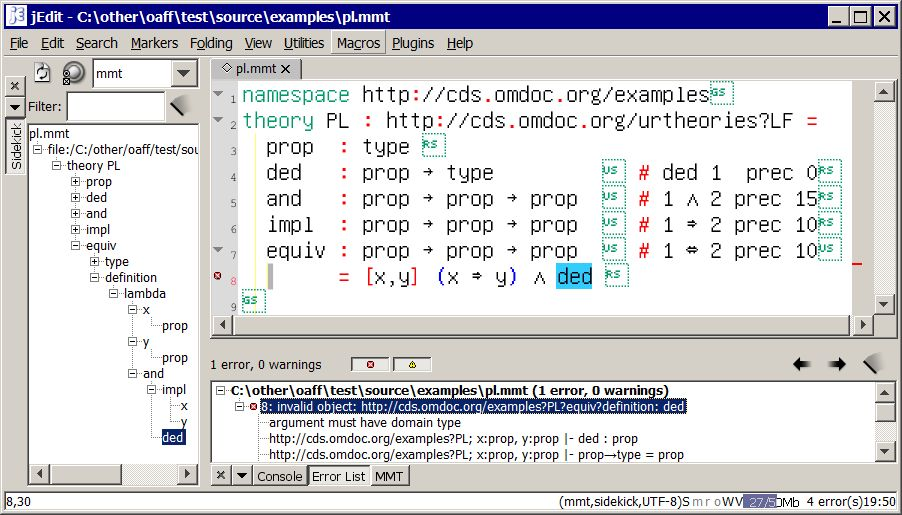
\includegraphics[width=\textwidth]{img/jedit-sidebar-errors.jpg}
\end{frame}

\begin{frame}\frametitle{An Interactive Library Browser}
\begin{itemize}
\item MMT content presented as HTML5+MathML pages
%\\[.5cm]
%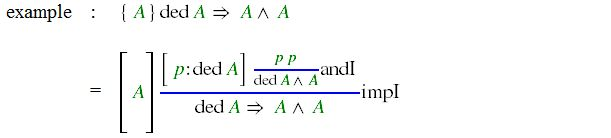
\includegraphics[width=\textwidth]{img/web-proof-tree.jpg}
%\\[.5cm]
\item Dynamic page updates via Ajax
\item MMT used through HTTP interface with JavaScript wrapper
\item Features
  \begin{itemize}
    \item interactive display
      \lec{e.g., inferred types, redundant brackets}
    \item smart navigation via MMT ontology
       \lec{can be synchronized with jEdit}
    \item dynamic computation of content
       \lec{e.g., definition lookup, type inference}
    \item graph view: theory diagram as SVG
  \end{itemize}
\end{itemize}
\end{frame}


\begin{frame}\frametitle{Browser: Example View}
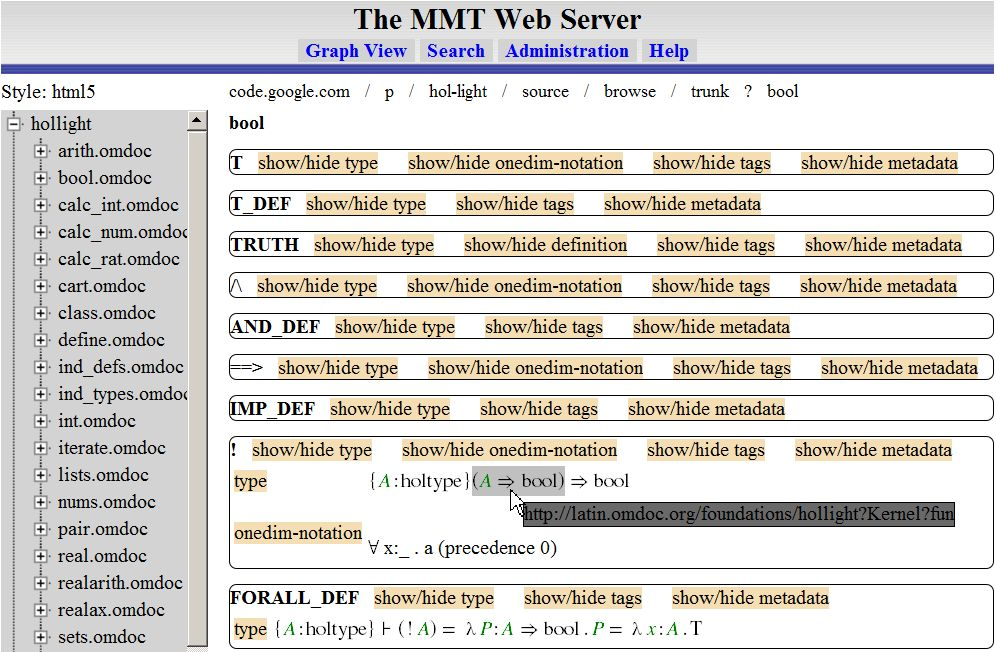
\includegraphics[width=\textwidth]{img/browse.jpg}
\end{frame}

\begin{frame}\frametitle{Browser Features: 2-dimensional Notations}
\begin{itemize}
\item Notations may use presentation MathML for complex renderings
\item Here: a fragment of the HOL Light library in the browser
\end{itemize}

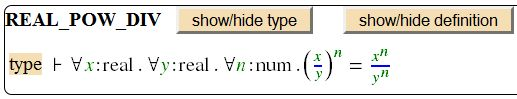
\includegraphics[width=\textwidth]{img/2dnot.jpg}
\end{frame}

\begin{frame}\frametitle{Browser Features: Proof Trees}
\begin{itemize}
\item Notations are expressive enough to render proofs as trees
\item Here: example solutions for a logic course
\end{itemize}

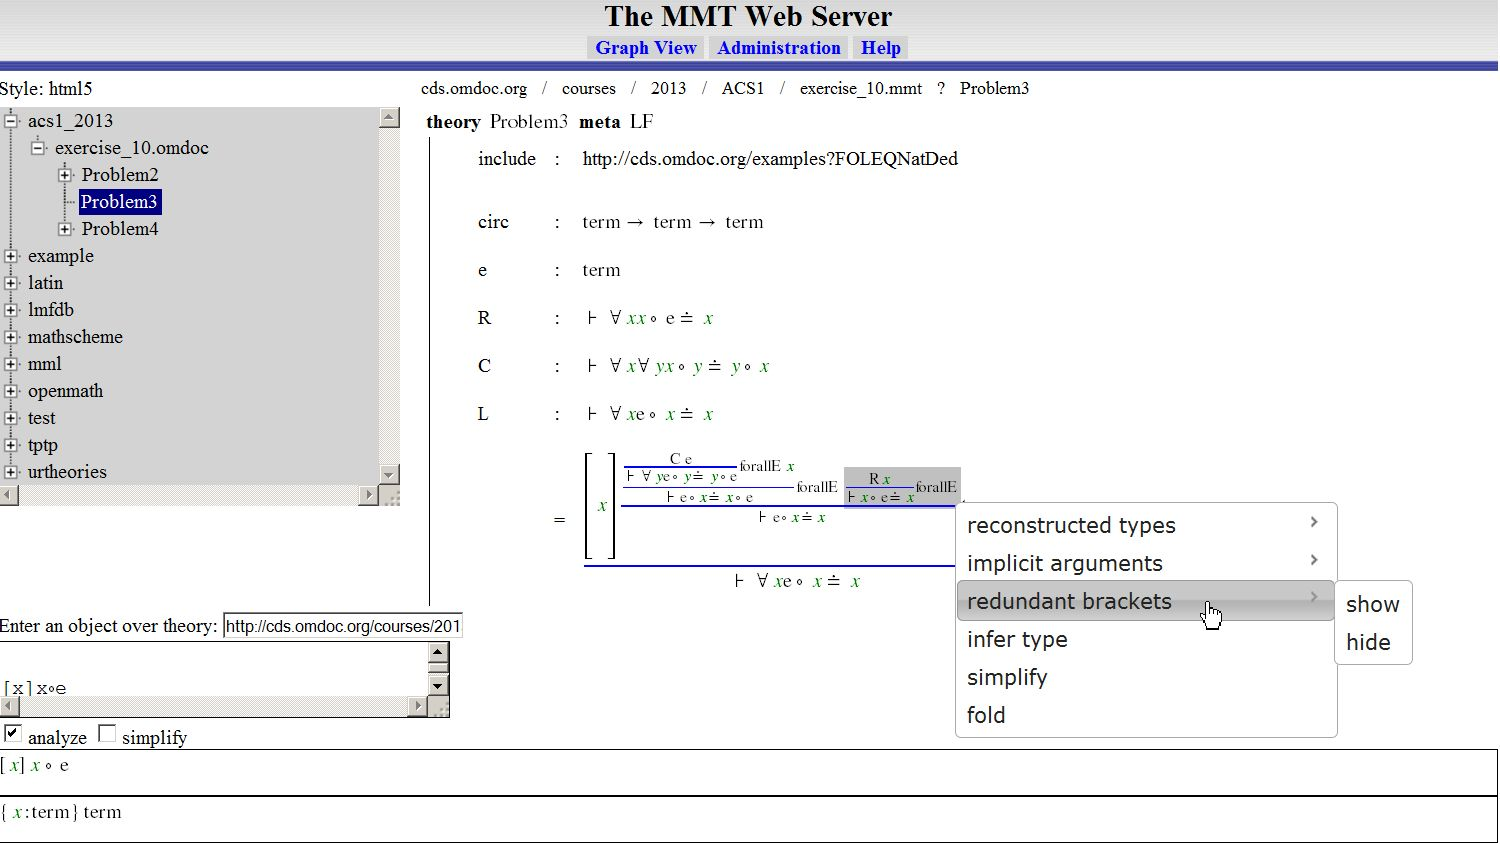
\includegraphics[width=\textwidth]{img/web-big.jpg}
\end{frame}

\begin{frame}\frametitle{Browser Features: Type Inferece}
\begin{itemize}
\item Interactive type inference for the selected subexpression
\item Here: definition of the polymorphic universal quantifier in MMT/LF/HOLLight
\end{itemize}

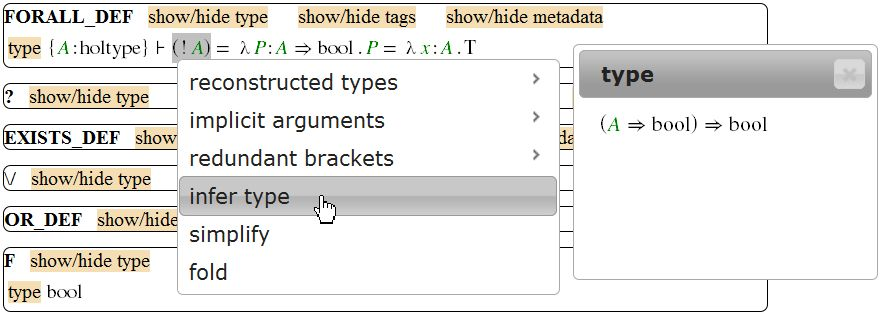
\includegraphics[width=\textwidth]{img/type-inference.jpg}
\end{frame}

\begin{frame}\frametitle{Browser Features: Parsing}
\begin{itemize}
\item Parser and checker can be easily integrated, e.g., into the web pages
\item Here:
 \begin{itemize}
 \item a simple formula in MMT/LF/HOLLight/Arith
 \item a text box with the formula (left)
 \item the rendering after parsing and analysis (right)
 \end{itemize}
\end{itemize}
\framebox{
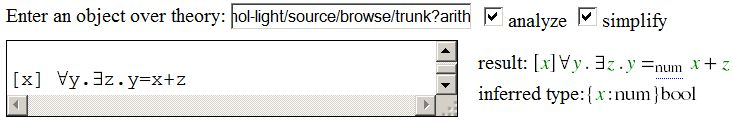
\includegraphics[width=\textwidth]{img/parse.jpg}
}
\end{frame}

\begin{frame}\frametitle{Example Service: Search}
A search query in the HOL Light library with $2$ example results:

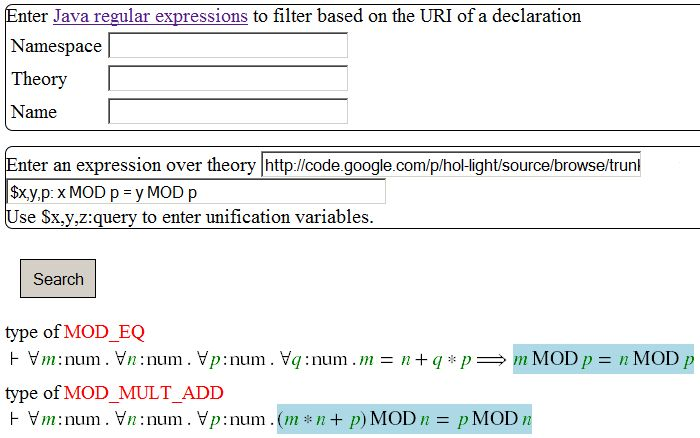
\includegraphics[width=\textwidth]{img/search.jpg}
\end{frame}

%
%\begin{frame}\frametitle{MMT and Hets}
%\begin{itemize}
%  \item Hets
%    \begin{itemize}
%      \item integration system for specification languages and associated tools
%      \item developed at DFKI by Till Mossakowski et al.
%      \item limited foundation-independence
%        \begin{itemize}
%          \item multiple foundations possible
%          \item but must be implemented individually
%        \end{itemize}
%    \end{itemize}
%  \item Integration
%    \begin{enumerate}
%     \item logics defined declaratively in MMT
%     \item MMT generates Hets logic definitions
%       \lec{includes logic-specific abstract data types}
%     \item new logics dynamically available in Hets
%   \end{enumerate}
%  \item Generated logics use MMT via HTTP for parsing/type-checking
%\end{itemize}
%\end{frame}

\begin{frame}\frametitle{\LaTeX Integration}
 \begin{itemize}
   \item MMT declarations spliced into {\LaTeX} documents
     \lec{shared MMT-{\LaTeX} knowledge space}
   \item {\LaTeX} macros for MMT-HTTP interface
   \item Semantic processing of formulas
    \begin{itemize}
     \item parsing
     \item type checking
     \item semantic enrichment: cross-references, tooltips
    \end{itemize}
  \item Design not \LaTeX-specific
   \lec{e.g., integration with word processors possible}
 \end{itemize}
\end{frame}

\begin{frame}\frametitle{\LaTeX Integration: Example}
Inferred arguments are inserted during compilation:
\begin{itemize}
\item upper part: \LaTeX\ source for the item on associativity
\item lower part: pdf after compiling with \LaTeX-MMT
\item type argument $M$ of equality symbol is inferred and added by MMT
\end{itemize}
\medskip

\hrule\medskip

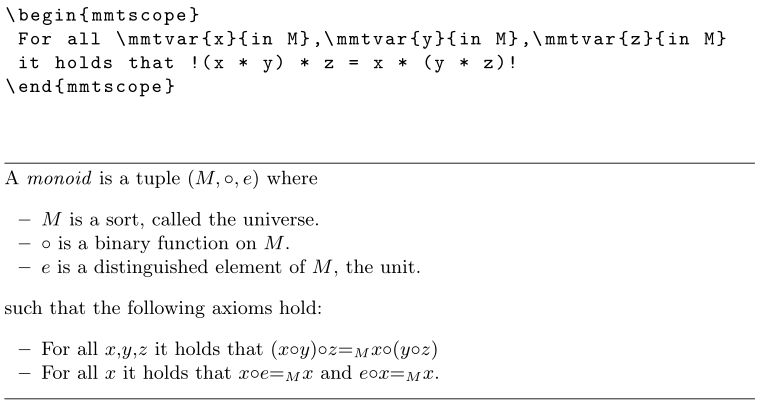
\includegraphics[width=\textwidth]{img/latex-mmt.jpg}
\thispagestyle{empty}
\end{frame}

%\begin{frame}\frametitle{MMT in the Semantic Alliance System}
%\begin{itemize}
% \item Semantic Alliance System
%   \begin{itemize}
%     \item developed by Michael Kohlhase et al.
%     \item two DFG projects
%		   \begin{itemize}
%		    \item SiSSi (Hutter, Kohlhase)
%		      \lec{spreadsheet applications}
%		    \item FormalCAD (Kohlhase, Schr\"oder)
%		      \lec{CAD applications}
%		   \end{itemize}
%	\end{itemize}
% \item Enrich domain-specific applications with semantic services
% \item Ontology used to
%   \begin{itemize}
%    \item formalize background knowledge
%    \item share knowledge between applications
%   \end{itemize}
% \item MMT used as interface to ontology
%\end{itemize}
%\end{frame}

%\begin{frame}\frametitle{Universal Representation Language}
%\begin{itemize}
% \item So far: MMT focuses on declarative formal languages
% \item Goal: extend to informal/natural language
%	   \begin{itemize}[<2>]
%	    \item practical specifications rarely fully formal
%	    \item partial formalization: formalize only important parts
%	      \lec{less expensive, more realistic}
%	    \item partial validation via MMT
%	      \lec{graceful degradation to informal knowledge}
%      \item state: new PhD student at Jacobs Univ.
%	      %\lec{state of the art for specifications in practice}
%	\end{itemize}
% \item Goal: extend to programming languages
%  \begin{itemize}[<3>]
%    \item share declarative aspects
%       \lec{class diagram = theory diagram}
%    \item first case study: MMT + Scala
%      \begin{itemize}
%        \item MMT theories compiled to Scala classes
%        \item Scala implementations reflected as MMT theories
%      \end{itemize}
%    \item Bridge natural and programming language
%     \begin{itemize} 
%       \item program snippets $\approx$ informal snippets
%       \item MMT maintains syntax, may be unaware of semantics
%     \end{itemize}
%  \end{itemize}
%\end{itemize}
%\end{frame}

%\begin{frame}\frametitle{Universal System Integration: MMT as Mediator}
%\begin{itemize}
% \item Typical:
%   \begin{itemize}
%     \item isolated paradigm-\alert{specific} applications
%     \item with overlapping knowledge bases
%       \begin{itemize}
%         \item informal -- word processor -- specification
%         \item programming -- compiler -- implementation
%         \item logical -- theorem prover -- formalization
%       \end{itemize}
%   \end{itemize}
% \item MMT approach: paradigm-\alert{independence}
%   \begin{itemize}
%     \item MMT maintains shared knowledge space across tools
%     \item tools register reusable knowledge fragments with MMT
%       \lec{export as MMT theories}
%		  \begin{itemize}
%		    \item informal language: partial formalization
%		    \item programming language: function headers but not bodies
%		    \item logic: theorems but not proofs
%		  \end{itemize}
%	 \end{itemize}
% \item Goal: semantics-aware tool integration \\
%       while maintaining existing work flows
%\end{itemize}
%\end{frame}
%
%\begin{frame}\frametitle{Universal System Integration: MMT as Interface Generator}
%\begin{itemize}
% \item Similar to parser/interface generation frameworks
%   \lec{e.g., UML, Protocol Buffers}
% \item But generalized to logic/type theory
% \item Formalize theory diagram in MMT
%   \begin{itemize}
%     \item declarative
%     \item foundation-independent
%   \end{itemize}
% \item Export theory diagram to peripheral tools
%     \lec{part of MMT build tool}
%   \begin{itemize}
%     \item foundation-specific tools
%     \item {\LaTeX} packages
%     \item class diagrams, (de)serialization code
%     \item testing code \lec{generated from axioms}
%     \item documentation website
%   \end{itemize}
% \item Goal: synchronize knowledge bases through central definition
%\end{itemize}
%\end{frame}

%\begin{frame}\frametitle{Interface Generation: Example}
%\begin{itemize}
% \item LMFDB
%   \begin{itemize}
%     \item collaboration of $\sim 40$ mathematicians in number theory
%     \item goal: integrate multiple related but isolated knowledge bases
%   \end{itemize}
% \item Problems
%  \begin{itemize}
%    \item semantic relations often unclear
%    \item incompatible encodings for knowledge exchange
%  \end{itemize}
% \item Planned use of MMT:
%    \begin{enumerate}
%     \item mathematicians define central theories in MMT
%       \lec{close to mathematical language due to foundation-independence}
%     \item MMT generates
%       \begin{itemize}
%         \item interface classes
%         \item testing functions
%         \item database schemata
%         \item encoding/decoding functions
%         \item documentation websites
%       \end{itemize}
%   \end{enumerate}
%\end{itemize}
%\end{frame}

\section{OAF: An Open Archive of Formalizations}

\begin{frame}\frametitle{Current Work: Library Integration}
 \begin{itemize}
 \item Open Archive of Formalizations  \hfill \emph{open PhD positions!}
   \lec{Michael Kohlhase and myself, 2014-2017}
 \item Goal: archival, comparison, integration of formal libraries
   \lec{Mizar, HOL systems, IMPS, Coq/Matita, PVS, \ldots}
 \item Big, overlapping libraries -- that are mutually incompatible
 \end{itemize}
 \begin{center}
 \framebox{
 \begin{tikzpicture}
 \node (MMT) at (3,1.5) {MMT};
 \node (L) at (2,0.5) {LF};
 \node (Lx) at (4,0.5) {LF+X};
 \draw[arrow](MMT) -- (L);
 \draw[arrow](MMT) -- (Lx);

 \draw[fill=red!60] (2,-.5) ellipse (3.2cm and .6cm);
 \node[color=red] at (-3.3,-.5) {LATIN logic library};
 \node at (2,-.7) {\ldots};

 \draw[fill=blue!60] (0,-2.25) ellipse (1.9cm and .8cm);

 \node (H) at (0,-.5) {HOL Light};
 \node[color=blue!80] at (-3.5,-2) {HOL Light library};
 \node (B) at (-1,-2) {Bool};
 \node (A) at (1,-2) {Arith};
 \node (E) at (0,-2.5) {\ldots};
 \draw[arrow](L) -- (H);
 \draw[arrow](H) -- (B);
 \draw[arrow](H) -- (A);
 \draw[arrow](B) -- (A);

 \draw[fill=olive] (4,-2.25) ellipse (1.9cm and .8cm);

 \node (M) at (4,-.5) {Mizar};
 \node[color=olive] at (-3.3,-2.5) {Mizar library};
 \node (B') at (3,-2) {XBoole};
 \node (A') at (5,-2) {XReal};
 \node (E') at (4,-2.5) {\ldots};

 \node (A) at (1,-2) {Arith};
 \node (E) at (0,-2.5) {\ldots};
 \draw[arrow](L) -- (M);
 \draw[arrow](M) -- (B');
 \draw[arrow](M) -- (A');
 \draw[arrow](B') -- (A');
 \end{tikzpicture}
 }
 \end{center}
 \thispagestyle{empty}
\end{frame}

\begin{frame}\frametitle{Goal: Universal Library Infrastructure}
\begin{itemize}
\item MMT as representation language
\item Repository backend: MathHub
 \begin{itemize}
  \item based on GitLab -- open-source analog of GitHub server
  \item GitLab instance hosted at Jacobs University
  \item free registration of accounts, creation of repositories
 \end{itemize}
\item Generic library management
 \begin{itemize}
  \item browser
  \item inter-library navigation
  \item search
  \item change management
\end{itemize}
\end{itemize}
\end{frame}

\begin{frame}\frametitle{Goal: Exports from Proof Assistants}
\begin{itemize}
\item Export major libraries into MMT
\item Representative initial targets
 \begin{itemize}
  \item Mizar: set theoretical
   \lec{initial export done (with Josef Urban)}
  \item HOL Light: higher-order logic
   \lec{initial export done (with Cezary Kaliszyk)}
  \item Coq or Matita: type theoretical
  \item IMPS: little theories method
  \item PVS: rich foundational language
\end{itemize}
\item Major technical difficulty
  \begin{itemize}
    \item exports must be written as part of proof assistant
    \item not all information available
  \end{itemize}
\end{itemize}
\end{frame}

\begin{frame}\frametitle{Goal: Towards Library Integration}
\begin{itemize}
\item Refactor exports to introduce modularity
\item 2 options
 \begin{itemize}
  \item systematically during export
   \lec{e.g., one theory for every HOL type definition}
  \item heuristic or interactive MMT-based refactoring
 \end{itemize}
\item Collect correspondences between concepts in different libraries
  \lec{heuristically or interactively}
\item Relate isomorphic theories across languages 
\item Use partial morphisms to translate libraries
\end{itemize}
\end{frame}

\section{}

\begin{frame}\frametitle{Conclusion}
\begin{itemize}
\item MMT: general framework for declarative languages
  \begin{itemize}
     \item Foundation-independent representation language
     \item Application-independent implementation
  \end{itemize}
\item Easy to instantiate with specific foundations
   \lec{rapid prototyping logic systems}
\item Multiple deep foundation-independent results
   \begin{itemize}
   \item logical: parsing, type reconstruction, module system, \ldots
   \item knowledge management: search, browser, IDE, \ldots
   \end{itemize}
\item MMT quite mature now, ready for larger applications \lec{about to break even}
\item Interesting for
 \begin{itemize}
  \item new, changing foundations
  \item generic applications/services
  \item system integration/combination
 \end{itemize}
\end{itemize}
\end{frame}

\end{document}


% frame templates
\begin{frame}\frametitle{}
\begin{itemize}
\item 
\item 
\item 
\item 
\end{itemize}
\end{frame}

\begin{frame}[fragile]\frametitle{}
\begin{lstlisting}
\end{lstlisting}
\end{frame}

\framebox{
\begin{tikzpicture}
\node[circle,draw] (A) at (1,0)
    {$A$};
\node (B) at (5,0)
    {$B$};
\node (C) at (9,0)
    {$C$};
\node (c) at (5,2) {$c$};
\node (i) at (-1,1) {$i$};
\draw[-triangle 45](A) -- node[above] {$f$} (B);
\draw[-](B) -- node[above] {$a$} (C);
\draw[->](A) .. controls (c) .. (C);
\draw[<-](A) .. controls (i) and (-1,-1) .. (A);
\end{tikzpicture}
}
